\documentclass{ximera}  
\title{Dynamic Programming}  
\pgfplotsset{compat=1.15}
\begin{document}  
\begin{abstract}  
We give an introduction to dynamic programming techniques via examples.
\end{abstract}  
\maketitle

\section{Dynamic Programming}

In the Recursion section, we defined the Fibonacci sequence recursively as $$f_n=\begin{cases} 1 & \text{if $n=0,1$}\\ f_{n-1}+f_{n-2} & \text{otherwise.}\end{cases}$$ Additionally, we presented the following code to compute these values:
\begin{sageCell}
def fib(n):
        if n < 2:
                return 1
        else:
                return fib(n-1) + fib(n-2)			
fib(5)
\end{sageCell}
While the function for \verb|fib| is very short and easy to read, it does suffer from one major drawback. If you try to compute \verb|fib(100)| you will find that the computer will complain and not be able to do it. Why? Because to compute \verb|fib(100)|, the program will first attempt to compute \verb|fib(99)| before computing \verb|fib(98)| and adding those values together. But to compute \verb|fib(99)| it will first compute \verb|fib(98)| before computing \verb|fib(97)| and so on. So you can see that the program is giving the computer a lot of needless work. The program ends up computing the same values multiple times because it never ``remembers" that it already did the same work before. A better approach would be to start from the beginning and work our way up to the desired term in the sequence. We write down, in a list or table, the terms of the sequence as we compute them. If we ever need them again, we just look to our table of computed values rather than recomputing them (which can waste a lot of time). Below is an example of this approach:
\begin{sageCell}
def dyn_fib(n):
        if n < 2:
                return 1
        else:
                L = [0 for i in range(n)]
                L[0] = 1
                L[1] = 1
                for i in range(2,n):
                        L[i] = L[i-1]+L[i-2]
                return L[-1]
dyn_fib(100)
\end{sageCell}

What we are really doing here is trading computational time for space on your computer's memory. We spend less time computing the desired value by avoiding duplicate work, but we require enough space in memory to hold all of the values we may need. This is what is referred to as a dynamic programming approach. Dynamic programming can work well whenever you have a problem whose solution can be determined by first solving sub-problems of the same type and then combining those solutions to solve the original problem. In the case of the Fibonacci sequence, the value of $f_n$ is clearly related to prior values of the sequence, $f_{n-1}$ and $f_{n-2}$, when $n\geq 2$. (Note: We do not actually need dynamic programming for the Fibonacci sequence, but it makes for an easier example to use as an introduction.)

Once we decide to use dynamic programming to solve a problem, such solutions typically involve a few steps:
\begin{enumerate}
	\item We must create a list or table where each entry will contain the solution to some related sub-problem.
	\item We must populate the list with solutions to initial cases (for recursively defined functions this would be the base cases).
	\item We must determine what relationship exists between the list or table entries in order to populate the rest of the list without doing any duplicate work.
\end{enumerate}

In the case of the Fibonacci sequence, our second solution applied the above steps in the following way:
\begin{align*}
	L\text{ is a list of length $n$}\\

	L[i]\text{ is ith Fibonacci number}\\

L[0],L[1] = 1

	L[i] = L[i-1] + L[i-2]\text{ for $i \geq 2$}
\end{align*}

\section{Examples}

In this section we illustrate how to use dynamic programming via several examples.

\subsection{The Lightbulb Problem}

Suppose that a company sells lightbulbs in packages of size 1, 2, 6, and 8. If a customer orders 30 lightbulbs, what is the least number of packages (of any size) that can be used to put this order together?

We begin with an simple approach. How many packages would we have to use if we simply tried using the largest package available at the time? In this case we would end up using 3 packages of size 8 and one of size 6. This is optimal here, but this strategy does not always work. (Try applying this same strategy to an order of 12 lightbulbs.)

To see how to use dynamic programming, let's work backwards. When putting an order of 30 lightbults together, we either:
\begin{enumerate}
	\item solved the problem for 22 bulbs and added a package of size 8, or 
	\item solved the problem for 24 bulbs and added a package of size 6, or 
	\item solved the problem for 28 bulbs and added a package of size 2, or 
	\item solved the problem for 29 bulbs and added a package of size 1.
\end{enumerate}
So if we could first solve the problem for 22, 24, 28, and 29, we could solve the problem for 30 by finding the minimum solution out of those 4 problems and adding 1 (for the additional package needed to get to 30). Working backwards this way we see that we would also need to solve some initial cases, namely 1 to 8 would do. So we will establish a list of values that will track our sub-problem solutions together with some initial cases and the relationship between entries in our list.
\begin{verbatim}
==============================
L is a list of length n

L[i] is the minimum number of packages 
     needed to put together a lightbulb order of size i

L[1] = 1, L[2] = 1, L[3] = 2, L[4] = 2, 
L[5] = 3, L[6] = 1, L[7] = 2, L[8] = 1

L[i] = min(L[i-8], L[i-6], L[i-2], L[i-1]) + 1 for i >= 9
==============================
\end{verbatim}

We apply the above algorithm in the SageCell below. Two notes are needed here. We use \verb|N = max(8,n)| in place of \verb|n| to avoid issues when \verb|n| is smaller than 8 and we add an extra item in our list since lists are zero-indexed in Python.

\begin{sageCell}
def bulb(n):
        N = max(8,n)
        L = [0 for i in range(N+1)]
        L[1] = 1
        L[2] = 1
        L[3] = 2
        L[4] = 2
        L[5] = 3
        L[6] = 1
        L[7] = 2
        L[8] = 1
        for i in range(9,N+1):
                L[i] = 1 + min(L[i-8], L[i-6], L[i-2], L[i-1])
        return L[n]
bulb(30)
\end{sageCell}

\subsection{Maze Solver}

Suppose we are given a rectangular ``maze" like the one below. Assume that we always start at the top left corner and always end at the bottom right corner. If we are only allowed to move down or to the right, how many different paths can we take to get to the end? Our goal is to count the number of distinct paths from the start to the end of the maze. Consider the following example:

\begin{center}
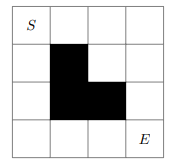
\includegraphics{maze_example.png} 
\end{center}

The number of distinct paths from the start to the end of this maze is 3.

\begin{center}
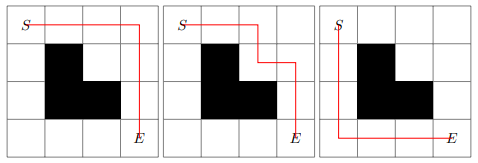
\includegraphics{maze_example_solutions.png}
\end{center}

From this point on, mazes will be encoded as a matrix (a list of lists) where a 0 entry represents an open space in the maze and a -1 represents a blocked space in the maze. For example, the maze above is encoded as the following list:

\begin{verbatim}
==============================
maze = [[0, 0, 0, 0],
        [0,-1, 0, 0],
        [0,-1,-1, 0],
        [0, 0, 0, 0]]
==============================
\end{verbatim}

For each square in the maze, beginning with the start position, we can count the number of paths to that particular square by adding up the number of paths to the square above it and to the left (should they exist). In particular, we can solve the problem in the following way:
\begin{verbatim}
==============================
maze is a matrix (list of lists) that determines the shape of our puzzle

M is a matrix (list of lists) that has the same dimensions as maze

M[0][0] = 1
M[0][j] = 0 if maze[0][j] = -1 and j > 0
M[0][j] = M[0][j-1] if maze[0][j] and j > 0

M[i][0] = 0 if maze[i][0] = -1 and i > 0
M[i][0] = M[i-1][0] if maze[i][0] and i > 0

M[i][j] = 0 if maze[i][j] = -1 and i,j > 0
M[i][j] = M[i-1][j] + M[i][j-1] if maze[i][j] = 0 and i,j > 0
==============================
\end{verbatim}

We implement the above in the SageCell below and apply it to our original maze.
\begin{sageCell}
def maze_solver(maze):
        # of rows in the original maze
        rows = len(maze)
        # of columns in the original maze
        columns = len(maze[0])
        # create matrix with zeros that has the same dimensions as maze
        M = [[0 for i in range(rows)] for j in range(columns)]
        # set first entry
        M[0][0] = 1
        # set first row
        for j in range(1,columns):
                if maze[0][j] == -1:
                        M[0][j] = 0
                else:
                        M[0][j] = M[0][j-1]
        # set first column
        for i in range(1,rows):
                if maze[i][0] == -1:
                        M[i][0] = 0
                else:
                        M[i][0] = M[i-1][0]
        # set remaining entries
        for i in range(1,rows):
                for j in range(1,columns):
                        if maze[i][j] == -1:
                                M[i][j] = 0
                        else:
                                M[i][j] = M[i-1][j] + M[i][j-1]
        # prints M (for testing)
        #for i in range(rows):
        #    print(M[i])
        # return bottom rightmost entry
        return M[-1][-1]

maze = [[0, 0, 0, 0],
        [0,-1, 0, 0],
        [0,-1,-1, 0],
        [0, 0, 0, 0]]

maze_solver(maze)
\end{sageCell}

\subsection{The Longest Subsequence}

Consider the following sequence of numbers: $$20,30,2,16,8,15,6,19,25,17.$$ How long is the longest subsequence of strictly increasing integers in this sequence?

Testing all possible subsequences would involve checking $2^{10}$ possible subsequences. Clearly, the brute force approach would fail if our sequence had, say, 100 terms. Taking a dynamic programming approach greatly reduces the amount of time needed to compute the solution. As usual, the trade-off is that we need to create a list that tracks the solutions to related sub-problems of our current problem and we have to come up with a relationship between answers on that list.

Consider the following sub-problem problem of the original question. How long is the longest subsequence of strictly increasing integers in the following sequence? $$20,30,2,16,8,15,6$$ A quick glance will show that the longest subsequence of strictly increasing integers is of length 3. If we append the number 19 to this sub-problem, how does it affect our previous answer? This depends on whether or not 19 is larger that the last element of any subsequence of length 3 in the original problem. With this idea in mind, what we will do is create a list that keeps track of the longest subsequence ending with each number in our original sequence. 

\begin{verbatim}
==============================
a is a sequence (list) of length n

a[i] = the ith term in the given sequence

L is a list of length n

L[i] = the length of the longest subsequence ending with a[i]

L[0] = 1

L[i] = 1 + max(L[j] if a[j] < a[i]) for i > 0
==============================
\end{verbatim}
Applying this idea to the sub-problem of the original problem, we have that:
\begin{center}
	\begin{tabular}{|c|c|c|c|c|c|c|c|c|}
		\hline
		\verb|i| & 0 & 1 & 2 & 3 & 4 & 5 & 6 & 7\\
		\hline
		\verb|a[i]| & 20 & 30 & 2 & 16 & 8 & 15 & 6 & 19 \\
		\hline
		\verb|L[i]| &  1 &  2 & 1 &  2 & 2 &  3 & 2 & 4 \\
		\hline
	\end{tabular}
\end{center}
To see how \verb|L[7]| is computed, note that in this case \verb|a[7]|=19, so \verb|L[7]| is one more than the maximum out of \verb|L[2]|, \verb|L[3]|, \verb|L[4]|, \verb|L[5]|, and \verb|L[6]|. This immediately gives that \verb|L[7]| is 4. What this result is saying is that there is a subsequence of length 4 ending with 19 because we found a subsequence of length 3 that ended with a number smaller than 19. In fact, this is the longest subsequence ending with 19.

Continuing in this way, we see that the solution to the original problem is that the longest subsequence of strictly increasing integers has length 5.

\subsection{The 0/1 Knapsack Problem}

In this problem, we consider the following situation. Suppowe we have a knapsack (or backpack, if you prefer) with a weight limit of 10 lbs. We also have the following 6 items available:
\begin{enumerate}
	\item a 1 lb. can of caviar that costs \$20,
	\item a 2 lb. bottle of water that costs \$5,
	\item a 3 lb. bag of trail mix that costs \$10,
	\item an 8 lb. bag of coffee that costs \$40,
	\item a 7 lb. bag of chicken that costs \$15, and
	\item a 4 lb. container of butane that costs \$25.
\end{enumerate}
Given the choice of items above and the 10 lb. restriction on the knapsack, what is the maximum value (in \$) worth of items that can be held in the knapsack? (Note: This problem is known as the 0/1 knapsack problem because you can think of making a binary choice for each item. You can choose to put the item in the knapsack, designated by a 1, or leave the item behind, designated by a 0.)

The approach for this problem is somewhat similar to that used for finding the longest increasing subsequence. We will first try to maximize the value using only the first item for knapsacks with weight limits of $0,1,2,\dots,10$ lbs. We will then see if we can improve our previous results if we are also allowed to use the second item. We will then add the third and so on until we find the answer to the original problem. (The order of the items does not matter here. There is no need to sort the items by weight or value or any other measure.)

It should be clear that when using just the first item, the maximum value that can be held by the knapsack is \$20 once the knapsack can hold at least 1 lb. If we now allow the second item to be considered, it should be clear that our new answers should never be any smaller than they were before for all of the different knapsack weight limits. If the knapsack can hold at most 1 lb., then our current best is still \$20. If the knapsack can hold 2 lbs. then we have a choice: either the knapsack holds \$20 as before, or we can add \$5 to whatever the knapsack could hold when it still had room for the second item. In this case, for the knapsack with a weight limit of 2 lbs. we must have had 0 lbs. worth of stuff in it (worth \$0) before using the new item. So here, again, it is better to not use the second item. If the knapsack can hold at least 3 lbs., then using the same reasoning as for the 2 lb. case we see that the knapsack can hold \$25 worth of items.

Continuing in this way will give the overall solution to the problem. As we consider more items (one at a time), we are really updating prior solutions. We have to ask ourselves if it is better to simply use our previous best answer, or see if we can do better by leaving enough room (in terms of weight) for the new item considered. With this in mind we define our matrix to help us solve this problem in the following way:

\begin{verbatim}
==============================
W is the maximum weight the knapsack can hold

c is the sequence (list) of item costs

c[i] = the cost of the ith item

w is the sequence (list) of item weights

w[i] = the weight of the ith item

M is a matrix (list of lists) with i rows and W+1 columns

M[i][j] = the maximum value that can be held by a knapsack
          with a maximum weight limit of j if we only consider
          using items 0, 1, 2, ..., i

M[i][0] = 0 for all i

M[0][j] = 0 if j < w[0]
M[0][j] = c[0] if j >= w[0]

M[i][j] = M[i-1][j] if j < w[i] for i > 0
M[[i][j] = max(c[i] + M[i-1][j-w[i]], M[i-1][j]) if j >= w[i] for i > 0
==============================
\end{verbatim}
The line \verb|M[[i][j] = max(c[i] + M[i-1][j-w[i]], M[i-1][j])| may be initially somewhat confusing, so we give additional details here to (hopefully) provide some clarification. If \verb|M[i][j]| represents the optimal solution when considering items \verb|0| to \verb|i| with a knapsack weight limit of \verb|j|, then this optimal solution could have only been obtained in one of two ways:
\begin{itemize}
	\item If we do not use item \verb|i|, then our optimal solution should be the same as the one when we considered items \verb|0| to \verb|i-1| with a weight limit of \verb|j| (since we are just doing what we did before), which is given by \verb|M[i-1][j]|.
	\item If we do use the item \verb|i|, then our optimal solution should be the cost of the new item, \verb|c[i]|, added to the optimal solution when we considered items \verb|0| to \verb|i-1|, but with a weight limit of \verb|j-w[i]| (if we want to use item \verb|i| with a weight limit of \verb|j|, then before putting item \verb|i| into the knapsack there must be enough room for it), which is given by \verb|M[i-1][j-w[i]]|.
\end{itemize}
Taking the maximum of these two options (as there are no other choices, you use the new item or you do not) gives the desired result.

We construct the table for \verb|M| in this case and then implement our solution in the SageCell below.

\begin{center}
	\begin{tabular}{|c|c|c|c|c|c|c|c|c|c|c|c|}
		\hline
	\verb|i|  & 0 & 1 & 2 & 3 & 4 & 5 & 6 & 7 & 8 & 9 & 10\\
		\hline
		\hline
	0 & 0  & 20  & 20  & 20  & 20  & 20  & 20  & 20  & 20  & 20  & 20  \\
		\hline
	1 & 0  & 20  & 20  & 25  & 25  & 25  & 25  & 25  & 25  & 25  & 25  \\
		\hline
        2 & 0  & 20  & 20  & 25  & 30  & 30  & 35  & 35  & 35  & 35  & 35  \\
		\hline
	3 & 0  & 20  & 20  & 25  & 30  & 30  & 35  & 35  & 40  & 60  & 60  \\
		\hline
	4 & 0  & 20  & 20  & 25  & 30  & 30  & 35  & 35  & 40  & 60  & 60  \\
		\hline
	5 & 0  & 20  & 20  & 25  & 30  & 45  & 45  & 50  & 55  & 60  & 60  \\
		\hline
	\end{tabular}
\end{center}

The table above can also be used to determine what items go into the knapsack, but that is beyond what we intend to accomplish here. 
\begin{sageCell}
def knapsack(W,w,c):
        M = [[0 for j in range(W+1)] for i in range(len(c))] # create matrix
        for j in range(w[0],W+1):                            
                M[0][j] = c[0]                               # fill in the first row values
        for i in range(1,len(c)):
                for j in range(1,W+1):
                        if j < w[i]:  
                                M[i][j] = M[i-1][j]          # use previous answer when knapsack limit is less than new item weight
                        else:
                                M[i][j] = max(c[i]+M[i-1][j-w[i]],M[i-1][j]) # compare using new item to otherwise
	#for i in M:           
	#        print(i)      # prints matrix
        return M[len(c)-1][W]

knapsack(10,[1,2,3,8,7,4],[20,5,10,40,15,25])
\end{sageCell}

We see now that in our original problem we can place \$60 worth of items into the knapsack. Note that we do not have to fill the knapsack to its weight limit to reach this optimal value.

\subsection{Minimum Insertions to Form a Palindrome}

A palindrome is a word that is spelled the same way forwards and backwards, like racecar or radar. Consider the following string of characters: $$aabcab.$$ What is the minimum number of characters that would need to be added to this string (in any location) to make it into a palindrome? You can quickly see that your answer should not be larger than 6, since $bacbaaaabcab$ is a palindrome, but can you do better than that?

Since the leftmost and rightmost letters of $aabcab$ do not match, then it must be the case that we will eventually have to add either a $b$ on the left end of the word or an $a$ on the right end of the word. In other words, we will first have to figure out the solution to the sub-problem $aabca$ and then add 1 insertion to handle the rightmost $b$ or we will have to figure out the solution to the sub-problem $aabcab$ and then add 1 insertion to handle the leftmost $a$. Note that if the leftmost and rightmost letters match, we instead drop these outside matching letters (since they are already in a good position) and solve the sub-problem for what remains. We summarize this approach as follows:

\begin{verbatim}
==============================
s is a string of characters of length n

s[i] is the ith character of the string

M is a matrix (list of lists) with n rows and n columns

M[i][j] = the minimum number of insertions needed to make the
          substring from the ith character to the jth 
          character a palindrome

M[i][j] = 0 if j > i

M[i][j] = 0 if i = j

M[i][j] = M[i+1][j-1] if s[i] = s[j] when i > j

M[i][j] = 1 + min(M[i+1][j],M[i][j-1]) if s[i] != s[j] when i > j
==============================
\end{verbatim}

We construct the table for \verb|M| for our example.

\begin{center}
	\begin{tabular}{|c|c|c|c|c|c|c|c|}
		\hline
		& $s_0$ & $s_1$ & $s_2$ & $s_3$ & $s_4$ & $s_5$\\
		\hline
		\hline
		$s_0$ & 0& 0& 1& 2& 2& 3\\
		\hline
		$s_1$ & 0& 0& 1& 2& 1& 2\\
		\hline
	        $s_2$ & 0& 0& 0& 1& 2& 1\\
		\hline
		$s_3$ & 0& 0& 0& 0& 1& 2\\
		\hline
	        $s_4$ & 0& 0& 0& 0& 0& 1\\
		\hline
	        $s_5$ & 0& 0& 0& 0& 0& 0\\
		\hline
	\end{tabular}
\end{center}

In the SageCell below we implement this approach in Python. Notice that this problem requires that we fill in the table along diagonals, rather than by row or column.

\begin{sageCell}
def minInsert(s):
        le = len(s)
        M = [[0 for j in range(le)] for i in range(le)]
        for k in range(1,le):
                for i in range(le-k):
                        j = k + i
                        if s[i] == s[j]:
                                M[i][j] = M[i+1][j-1]
                        else:
                                M[i][j] = 1 + min(M[i+1][j],M[i][j-1])
        #for m in M:
                #print(m)
        return M[0][-1]

minInsert('aabcab')
\end{sageCell}

So we see now that the minimum number of insertions is 3. As in the 0/1 knapsack problem, the table of values generated can be used to determine where the insertions were made. This is beyond what we intend to accomplish here, but in this case a palindrome (there are many) generated with a minimum number of insertions for our example is $baacbcaab$.

\section{Problems}

\begin{question}
Compute the number of ways to climb 50 stairs be either taking one stair or three stairs at once per step. (See question 3 from the Recursion section.) $\answer{178955183}$
\end{question}

\begin{question}
Suppose that a company sells bolts in packages of size 1, 6, and 7. Determine the minimum number of packages to buy 18 bolts. $\answer{3}$
\end{question}

\begin{question}
Determine the number of distinct paths from the start to the end of the following maze.
\begin{verbatim}
[[0, 0, 0,-1, 0, 0, 0, 0],
 [0,-1, 0, 0, 0, 0, 0, 0],
 [0,-1, 0, 0, 0, 0, 0, 0],
 [0,-1, 0,-1, 0, 0, 0, 0],
 [0,-1, 0, 0, 0, 0, 0, 0]]
\end{verbatim}
	$\answer{41}$
\end{question}

\begin{question}
Determine the solution to the 0/1 knapsack problem if your knapsack has a weight limit of 9 lbs. and you have 6 items with the following weights and costs:
	\begin{center}
		\begin{tabular}{|c|c|c|c|c|c|c|}
			\hline
			item & 0 & 1 & 2 & 3 & 4 & 5\\
			\hline
			\hline
			weight & 1 & 3 & 2 & 5 & 7 & 4\\
			\hline
			cost & 10 & 20 & 15 & 35 & 10 & 25\\
			\hline
	\end{tabular}
	\end{center}

	$\answer{65}$
\end{question}

\begin{question}
Determine the minimum number of insertions needed to make the following string a palindrome: $bccaba$. $\answer{2}$
\end{question}

\begin{question}
Can the number 24 be written as a sum of the numbers 7,3,2,5,8?
	\begin{hint}
This problem is similar to the 0/1 knapsack problem. Set up a table \verb|M| that has 5 rows (for each number available) and 25 columns (for the numbers 0 to 24). Now let \verb|M[i][j]| be 1 if \verb|j| can be represented as a sum of the first \verb|i| numbers available and 0 otherwise.

So in the first row, only one entry should be a 1, namely \verb|M[0][7]|. As you move into the second row, it should be the case that \verb|M[1][7]| should also be 1 (if you could get 7 before, then you can certainly get it now). What new numbers can you now get if 3 is also available? (There should be 2 more.)

Continue in this way to fill out the rest of the table.
	\end{hint}
	\begin{multipleChoice}
	\choice[correct]{No}
	\choice{Yes}
	\end{multipleChoice}
\end{question}

\section{Workspace}

\begin{sageCell}
# Use this cell to solve the above questions.
\end{sageCell}

\end{document}
